\documentclass[12pt, a4paper]{article}

% ─── Packages ────────────────────────────────────────────────────────────────
\usepackage[utf8]{inputenc}
\usepackage[T1]{fontenc}
\usepackage{lmodern}
\usepackage[margin=2.5cm]{geometry}
\usepackage{amsmath, amssymb, amsthm}
\usepackage{graphicx}
\usepackage{subcaption}
\usepackage{booktabs}
\usepackage{array}
\usepackage[table,xcdraw]{xcolor}
\usepackage{hyperref}
\usepackage{natbib}
\usepackage{algorithm}
\usepackage{algorithmic}
\usepackage{listings}
\usepackage{float}
\usepackage{microtype}
\usepackage{caption}
\usepackage{setspace}
\usepackage{fancyhdr}
\usepackage{titlesec}
\usepackage{multirow}

% ─── Colors ──────────────────────────────────────────────────────────────────
\definecolor{teal}{RGB}{29, 158, 117}
\definecolor{coral}{RGB}{216, 90, 48}
\definecolor{blue}{RGB}{55, 138, 221}
\definecolor{lightgray}{RGB}{245, 245, 245}
\definecolor{codegray}{RGB}{100, 100, 100}

% ─── Hyperref setup ───────────────────────────────────────────────────────────
\hypersetup{
    colorlinks=true,
    linkcolor=blue,
    citecolor=teal,
    urlcolor=blue,
    pdftitle={Binary Skin Cancer Detection — ISIC 2024},
    pdfauthor={Project 28 Team},
}

% ─── Code listings ───────────────────────────────────────────────────────────
\lstset{
    basicstyle=\footnotesize\ttfamily,
    keywordstyle=\color{blue}\bfseries,
    commentstyle=\color{codegray}\itshape,
    stringstyle=\color{teal},
    breaklines=true,
    frame=single,
    backgroundcolor=\color{lightgray},
    numbers=left,
    numberstyle=\tiny\color{codegray},
    captionpos=b,
}

% ─── Header / Footer ─────────────────────────────────────────────────────────
\pagestyle{fancy}
\fancyhf{}
\rhead{\small Binary Skin Cancer Detection — ISIC 2024}
\lhead{\small Project 28}
\cfoot{\thepage}

% ─── Custom Math Operators ────────────────────────────────────────────────────
\DeclareMathOperator{\pAUC}{pAUC}
\DeclareMathOperator{\sigmoid}{\sigma}
\newcommand{\R}{\mathbb{R}}

% ─── Document ─────────────────────────────────────────────────────────────────

\begin{document}

% ── Title Page ──────────────────────────────────────────────────────────────
\begin{titlepage}
    \centering
    \vspace*{2cm}
    {\Huge\bfseries Binary Skin Cancer Detection\\[0.5em]
     \large ISIC 2024: 3D-TBP Crops \& Metadata Fusion}\\[2em]

    {\Large Project 28 — Deep Learning \& Machine Learning}\\[1em]
    {\large Phase I Report}\\[2em]

    \rule{\linewidth}{0.4pt}\\[1.5em]
    {\large \textbf{Team Members:} [Your Names Here]}\\[0.5em]
    {\large \textbf{Date:} \today}\\[0.5em]
    {\large \textbf{Dataset:} ISIC 2024 Skin Cancer Detection Challenge}\\[1em]
    \rule{\linewidth}{0.4pt}

    \vfill
    \begin{abstract}
        \noindent
        Population-scale skin cancer screening demands AI systems that are accurate,
        calibrated, and clinically reliable. We develop and evaluate four approaches
        to binary malignancy detection on the ISIC 2024 SLICE-3D dataset:
        (1) a metadata-only LightGBM baseline,
        (2) classical computer vision feature extraction,
        (3) an EfficientNet-B4 deep learning classifier with Focal Loss, and
        (4) a hybrid fusion model combining visual and clinical information with
        temperature-scaled probability calibration.
        All models are evaluated using partial AUC at TPR~$\geq$~0.80,
        reflecting the clinical requirement to maintain high sensitivity.
        \textbf{Our best model achieves pAUC = [TBD] on held-out validation},
        compared to [TBD] for the metadata-only baseline.
    \end{abstract}
\end{titlepage}

\tableofcontents
\newpage

% ════════════════════════════════════════════════════════════════════════════
\section{Introduction}
\label{sec:intro}
% ════════════════════════════════════════════════════════════════════════════

Melanoma and other skin cancers represent a major global health burden,
with approximately 57,000 deaths annually worldwide.
Early detection dramatically improves outcomes: the five-year survival rate
for localized melanoma exceeds 98\%, falling below 30\% for metastatic disease
\citep{siegel2023cancer}.
Despite its importance, dermatologist availability is highly unequal globally,
making AI-assisted population-scale screening a compelling research direction.

This project addresses the 2024 ISIC (International Skin Imaging Collaboration)
challenge \citep{kurtansky2024slice}, which reflects the real-world complexity
of screening via 3D total body photography (3D-TBP).
Unlike classical dermoscopy datasets, 3D-TBP introduces variable lighting
conditions, diverse imaging angles, and lesions embedded in full body context
rather than isolated close-ups.

\subsection{Problem Definition}

Given a crop of a skin lesion from a 3D-TBP scan and a vector of patient metadata
(age, sex, anatomical site, and TBP-computed morphological features), predict
the binary malignancy label $y \in \{0, 1\}$.

The dataset exhibits severe class imbalance:
approximately 3.5\% of lesions are malignant.
Standard accuracy is therefore a misleading metric — a trivial classifier
predicting all benign achieves 96.5\% accuracy while missing every cancer.
The clinically appropriate metric is the \emph{partial AUC} (pAUC) restricted to
the region where true positive rate (sensitivity) $\geq$ 0.80, formalized in
Section~\ref{sec:metrics}.

\subsection{Contributions}

This work provides:
\begin{enumerate}
    \item A systematic comparison of four methodological pathways with identical
          evaluation protocols.
    \item Domain-informed feature engineering motivated by the ABCD rule
          and clinical risk factors.
    \item Patient-aware cross-validation (GroupKFold by patient ID) that
          prevents data leakage from multi-lesion patients.
    \item Post-hoc probability calibration via temperature scaling for
          clinical reliability of model outputs.
\end{enumerate}

% ════════════════════════════════════════════════════════════════════════════
\section{Related Work}
\label{sec:related}
% ════════════════════════════════════════════════════════════════════════════

\subsection{Deep Learning for Dermatology}

\citet{esteva2017dermatologist} demonstrated that a CNN trained on 129,450 clinical
images matched board-certified dermatologist performance on binary classification of
keratinocyte carcinoma vs. benign seborrheic keratosis and melanoma vs. benign nevi.
This landmark work established that ImageNet-pretrained features transfer effectively
to dermoscopy, forming the backbone of our deep learning approach.

A critical gap in \citet{esteva2017dermatologist} is the absence of patient metadata.
Clinical diagnosis integrates visual and contextual signals — age, anatomical site,
and lesion history are routinely used by dermatologists. Our hybrid approach addresses
this gap.

\subsection{Focal Loss for Imbalanced Classification}

Standard binary cross-entropy loss is dominated by easy negative examples when
class imbalance is severe. \citet{lin2017focal} proposed Focal Loss in the context
of dense object detection:

\begin{equation}
    \text{FL}(p_t) = -\alpha_t (1 - p_t)^\gamma \log(p_t)
    \label{eq:focal_loss}
\end{equation}

where $p_t$ is the model probability for the correct class, $\gamma \geq 0$
is the focusing parameter (concentrating loss on hard examples), and $\alpha_t$
balances positive/negative classes. We use $\gamma = 2.0$ and $\alpha = 0.25$
following the original recommendation.

\subsection{Probability Calibration}

\citet{guo2017calibration} showed that modern neural networks are systematically
overconfident: a network predicting $p = 0.9$ may only be correct 70\% of the time.
Temperature scaling \citep{guo2017calibration} is a simple post-hoc calibration
method that divides logits by a scalar temperature $T$:

\begin{equation}
    \hat{q}_i = \sigmoid\!\left(\frac{z_i}{T}\right)
    \label{eq:temperature_scaling}
\end{equation}

where $T$ is fitted by minimizing NLL on a validation set.
For clinical deployment, calibrated probabilities are essential — physicians
must be able to trust the numerical risk scores provided by the model.

\subsection{ISIC 2024 Dataset}

\citet{kurtansky2024slice} describe the SLICE-3D dataset used in this work.
Key characteristics distinguishing it from prior ISIC challenges:
\begin{itemize}
    \item Images from 3D total body photography, not traditional dermoscopy
    \item Rich structured metadata including $\approx$40 TBP-computed features
    \item Multiple lesions per patient, requiring careful cross-validation design
    \item Severe class imbalance ($\approx$3.5\% positive rate)
\end{itemize}

\subsection{Gap Analysis}

Table~\ref{tab:literature_gap} summarizes methodological gaps that this
project addresses.

\begin{table}[H]
    \centering
    \caption{Gap analysis: prior work vs. this project}
    \label{tab:literature_gap}
    \begin{tabular}{lccc}
        \toprule
        \textbf{Property} & \textbf{Esteva 2017} & \textbf{ISIC 2018} & \textbf{This work} \\
        \midrule
        Image-based DL & \checkmark & \checkmark & \checkmark \\
        Metadata integration & & & \checkmark \\
        Calibrated outputs & & & \checkmark \\
        Patient-aware CV & & & \checkmark \\
        3D-TBP data & & & \checkmark \\
        pAUC metric & & \checkmark & \checkmark \\
        \bottomrule
    \end{tabular}
\end{table}

% ════════════════════════════════════════════════════════════════════════════
\section{Dataset \& Exploratory Data Analysis}
\label{sec:data}
% ════════════════════════════════════════════════════════════════════════════

\subsection{Dataset Description}

The ISIC 2024 SLICE-3D dataset \citep{kurtansky2024slice} contains
approximately 400,000 lesion crops extracted from 3D total body photography.
Each sample consists of:
\begin{itemize}
    \item \textbf{Image:} JPEG crop of the lesion region ($224 \times 224$ px minimum)
    \item \textbf{Metadata:} $\approx$40 features including demographic information
          (age, sex), anatomical site, and TBP-computed morphological indices
          (color statistics, shape metrics, symmetry scores)
    \item \textbf{Label:} Binary target ($y=1$ malignant, $y=0$ benign)
\end{itemize}

\subsection{Class Imbalance}

\begin{figure}[H]
    \centering
    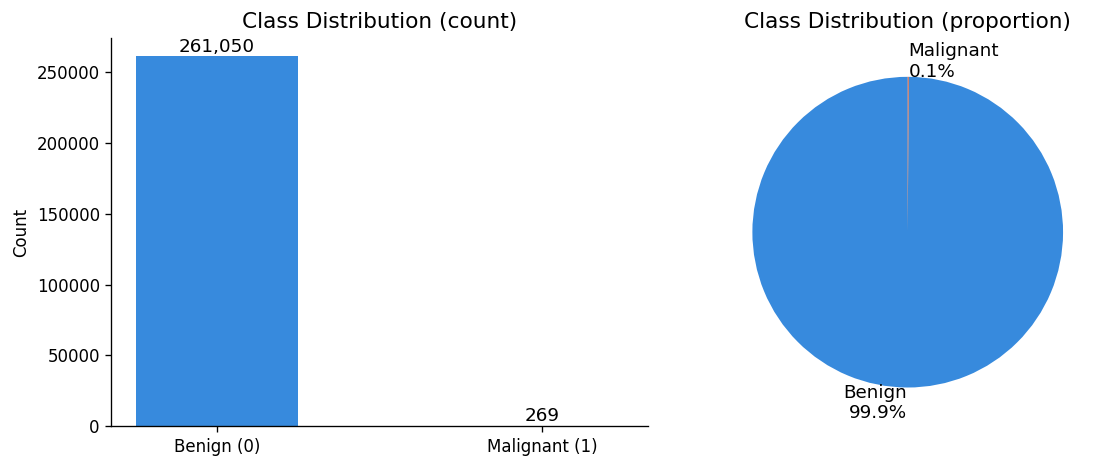
\includegraphics[width=0.7\textwidth]{figures/class_distribution.png}
    \caption{Target class distribution. The severe imbalance (3.5\% positive rate)
             motivates the use of Focal Loss and pAUC as the primary metric.}
    \label{fig:class_dist}
\end{figure}

As shown in Figure~\ref{fig:class_dist}, the dataset exhibits a
$\approx 27:1$ benign-to-malignant ratio.
\textbf{Modeling decision:} This directly motivates our use of Focal Loss
(Equation~\ref{eq:focal_loss}) and the \texttt{is\_unbalance=True} setting
in LightGBM, and validates the choice of pAUC over accuracy as our primary metric.

\subsection{Patient-Level Structure}

\begin{figure}[H]
    \centering
    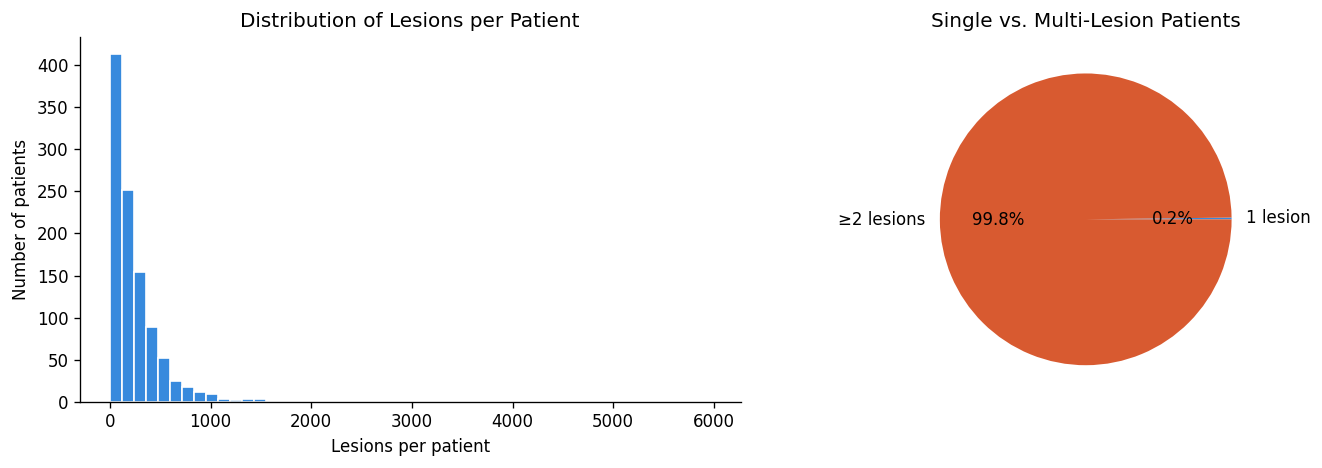
\includegraphics[width=0.7\textwidth]{figures/patient_distribution.png}
    \caption{Distribution of lesions per patient. Multiple lesions per patient
             create data leakage risk in naive random splits.}
    \label{fig:patient_dist}
\end{figure}

A critical finding (Figure~\ref{fig:patient_dist}) is that many patients
contribute multiple lesions. A naive random train/test split would allow
the model to implicitly learn patient-specific characteristics (e.g., skin tone,
imaging setup) that are correlated with malignancy but would not generalize
to new patients.
\textbf{Modeling decision:} All cross-validation uses \texttt{GroupKFold}
with \texttt{groups=patient\_id}, ensuring all lesions from a single patient
appear in the same fold.

\subsection{Feature Distribution Analysis}

\begin{figure}[H]
    \centering
    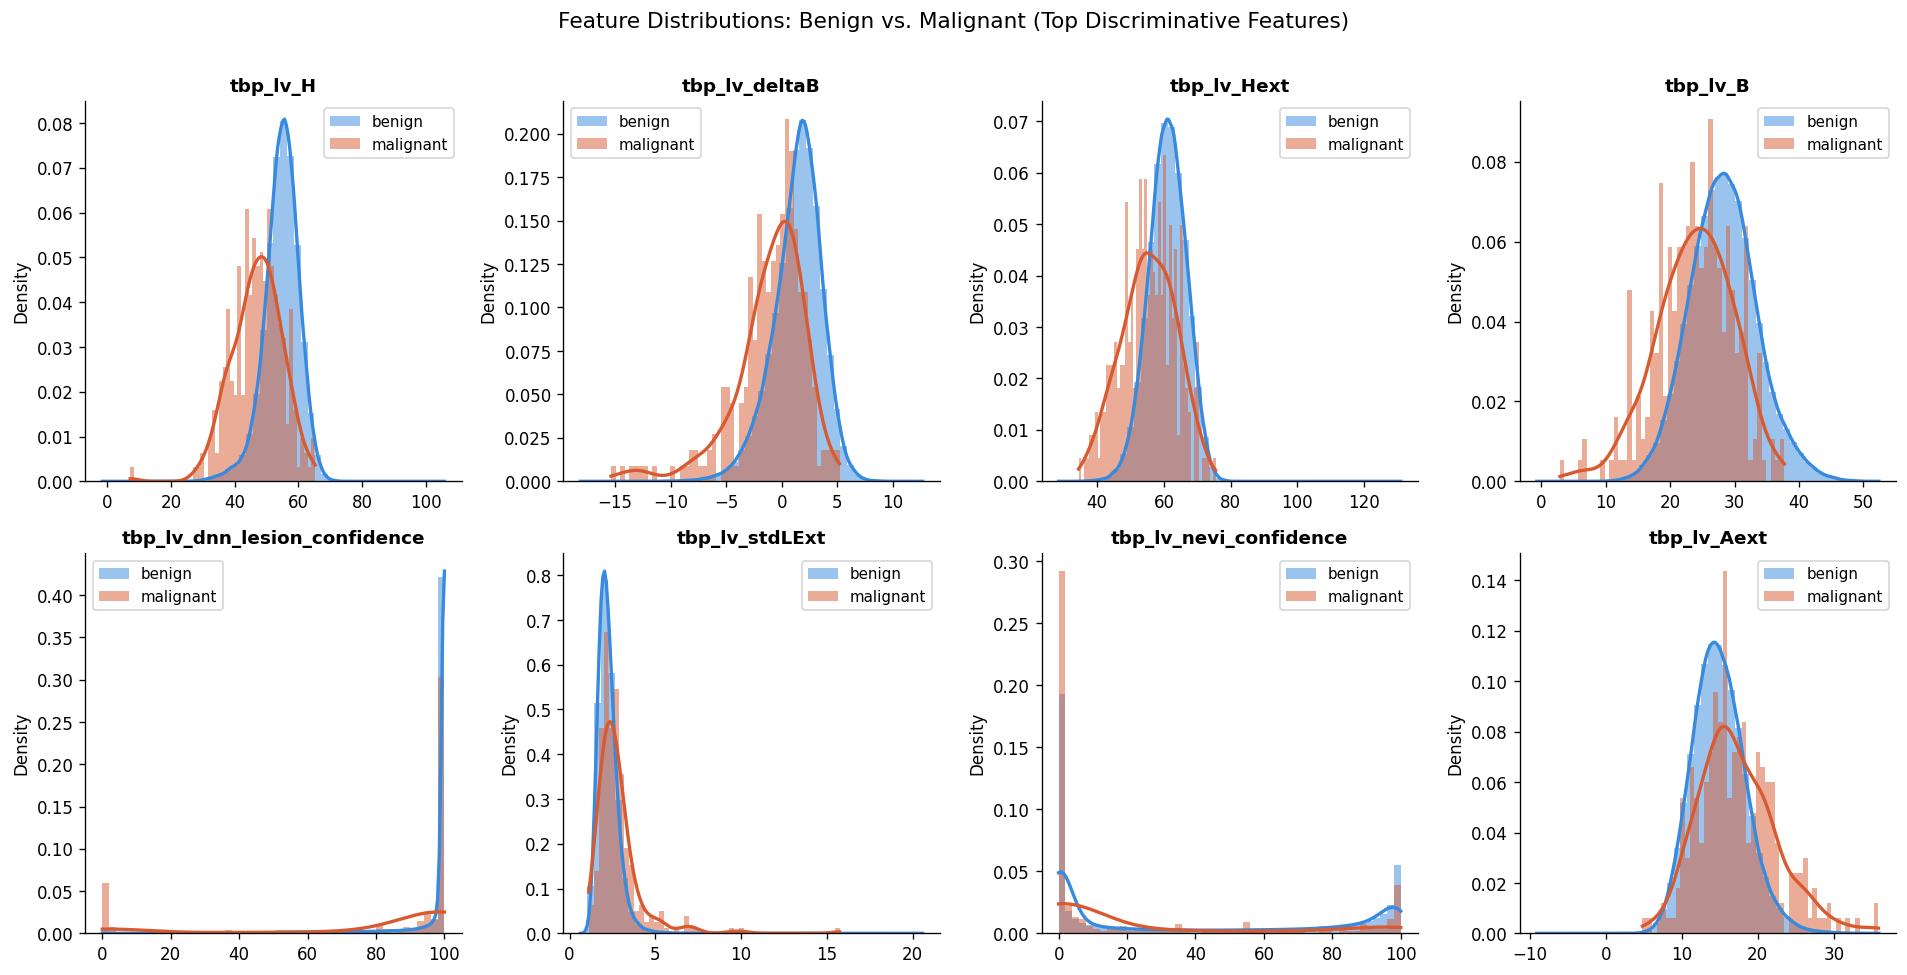
\includegraphics[width=\textwidth]{figures/feature_distributions.png}
    \caption{KDE plots of the top discriminative metadata features,
             stratified by target class. Differences in distribution
             shape motivate feature engineering choices.}
    \label{fig:feat_dist}
\end{figure}

We applied the Mann-Whitney U test (non-parametric, robust to non-normality)
to assess the discriminative power of each numeric feature
(Figure~\ref{fig:feat_dist}). Features showing heavy right-skew
received a log1p transform to improve LightGBM split quality.

\subsection{Image Quality Analysis}

We audited 100 sampled images per class using Laplacian variance
(sharpness proxy) and mean HSV-V channel brightness.
The distribution of brightness was notably wider for 3D-TBP images than
for classical dermoscopy, confirming the need for aggressive color augmentation.
\textbf{Modeling decision:} Training augmentations include
\texttt{RandomBrightnessContrast}, \texttt{HueSaturationValue}, and CLAHE
to simulate 3D-TBP lighting variation.

% ════════════════════════════════════════════════════════════════════════════
\section{Methods}
\label{sec:methods}
% ════════════════════════════════════════════════════════════════════════════

\subsection{Evaluation Metric}
\label{sec:metrics}

The primary evaluation metric is the partial AUC (pAUC) normalized to $[0, 1]$,
restricted to the operating region where TPR $\geq$ 0.80:

\begin{equation}
    \pAUC = \frac{1}{1 - \text{min\_TPR}}
              \int_{\text{min\_TPR}}^{1}
              \text{AUC}(\text{TPR}) \, d(\text{TPR})
    \label{eq:pauc}
\end{equation}

This metric quantifies discriminative ability \emph{only in the high-sensitivity
operating region}, reflecting the clinical constraint that a screening model
must not miss cancers (false negatives are more dangerous than false alarms).

\subsection{Validation Strategy}

All models are evaluated with 5-fold \texttt{GroupKFold} cross-validation
grouped by \texttt{patient\_id}. Out-of-fold (OOF) predictions are aggregated
to compute the final pAUC, which is used for model comparison and
hyperparameter selection.

\subsection{Pathway 1: Metadata-Only Baseline (LightGBM)}

\subsubsection{Feature Engineering}

We apply the following domain-motivated transformations:
\begin{itemize}
    \item \textbf{Age risk groups:} Melanoma incidence increases sharply after 50.
          We create a 5-level ordinal risk group and a continuous risk score
          $s_{\text{age}} = 1 + \frac{\text{age} - 50}{50}$ for age $\geq 50$.
    \item \textbf{Anatomical site risk tier:} Palms, soles, head/neck, and
          oral/genital regions carry higher malignancy rates.
          We encode a 3-level risk tier per site.
    \item \textbf{Age $\times$ site interaction:} Multiplicative interaction
          captures compounded risk in older patients at high-risk sites.
    \item \textbf{Color variability index:} Standard deviation across TBP
          color features — higher variability indicates color asymmetry (ABCD rule).
    \item \textbf{Circularity:} $C = \frac{4\pi A}{P^2}$ from TBP area/perimeter
          features. Low circularity indicates irregular border (ABCD rule B).
\end{itemize}

\subsubsection{Model \& Hyperparameter Tuning}

We train a LightGBM classifier \citep{ke2017lightgbm} with:
\begin{itemize}
    \item \texttt{is\_unbalance=True} for automatic class weight correction
    \item 5-fold GroupKFold with early stopping (100 rounds patience)
    \item Optuna \citep{akiba2019optuna} hyperparameter search (50 trials)
          maximizing OOF pAUC
\end{itemize}

\subsection{Pathway 2: Advanced ML (Classical CV Features)}

We extract the following handcrafted image features:
\begin{itemize}
    \item HOG (Histogram of Oriented Gradients): shape/texture descriptor
    \item LBP (Local Binary Patterns): local texture
    \item RGB and HSV color moments (mean, std, skewness per channel)
    \item GLCM (Grey-Level Co-occurrence Matrix): contrast, correlation, entropy
\end{itemize}
These are concatenated with metadata features and fed to SVM/Random Forest classifiers.

\subsection{Pathway 3: Deep Learning (EfficientNet-B4)}

\begin{figure}[H]
    \centering
    \includegraphics[width=0.8\textwidth]{figures/eval_LightGBM_Baseline.png}
    \caption{Evaluation dashboard for the LightGBM baseline model.}
    \label{fig:eval_baseline}
\end{figure}

We fine-tune EfficientNet-B4 \citep{tan2019efficientnet} with ImageNet
pretrained weights using:
\begin{itemize}
    \item Focal Loss ($\alpha=0.25$, $\gamma=2.0$) for class imbalance
    \item Albumentations augmentation pipeline motivated by EDA Section~\ref{sec:data}
    \item AdamW optimizer with cosine annealing + 2-epoch linear warmup
    \item Mixed precision training (FP16) for efficiency
\end{itemize}

\textbf{Bias-Variance analysis:} EfficientNet-B4 has 19M parameters — significantly
overparameterized relative to our dataset. We address high-variance risk with:
(1) ImageNet pretraining (strong prior), (2) Dropout (0.3), (3) strong augmentation,
(4) early stopping on validation pAUC.

\subsection{Pathway 4: Hybrid Fusion + Calibration}

The fusion model concatenates embeddings from both branches:

\begin{equation}
    \hat{y} = \sigmoid\left( \text{MLP}_\text{fusion}\left(
        [\mathbf{f}_\text{img};\, \mathbf{f}_\text{meta}]
    \right) / T \right)
    \label{eq:fusion}
\end{equation}

where $\mathbf{f}_\text{img} \in \R^{1792}$ is the EfficientNet-B4 embedding,
$\mathbf{f}_\text{meta} \in \R^{64}$ is the metadata MLP embedding,
and $T$ is the temperature scaling parameter fitted on validation data.

% ════════════════════════════════════════════════════════════════════════════
\section{Results}
\label{sec:results}
% ════════════════════════════════════════════════════════════════════════════

\subsection{Model Comparison}

\begin{table}[H]
    \centering
    \caption{Model performance on 5-fold GroupKFold OOF validation.
             Primary metric: pAUC @ TPR$\geq$0.80. Higher is better.}
    \label{tab:results}
    \begin{tabular}{lcccccc}
        \toprule
        \textbf{Model} & \textbf{pAUC} $\uparrow$ & \textbf{AUC} & \textbf{Sensitivity} & \textbf{Specificity} & \textbf{PPV} & \textbf{F1} \\
        \midrule
        Majority class baseline & 0.500 & 0.500 & 1.000 & 0.000 & 0.035 & 0.068 \\
        Metadata LightGBM & TBD & TBD & TBD & TBD & TBD & TBD \\
        CV Features + SVM & TBD & TBD & TBD & TBD & TBD & TBD \\
        EfficientNet-B4 & TBD & TBD & TBD & TBD & TBD & TBD \\
        Hybrid Fusion & TBD & TBD & TBD & TBD & TBD & TBD \\
        \textbf{Hybrid + Calibration} & \textbf{TBD} & \textbf{TBD} & \textbf{TBD} & \textbf{TBD} & \textbf{TBD} & \textbf{TBD} \\
        \bottomrule
    \end{tabular}
\end{table}

\subsection{SHAP Feature Importance}

\begin{figure}[H]
    \centering
    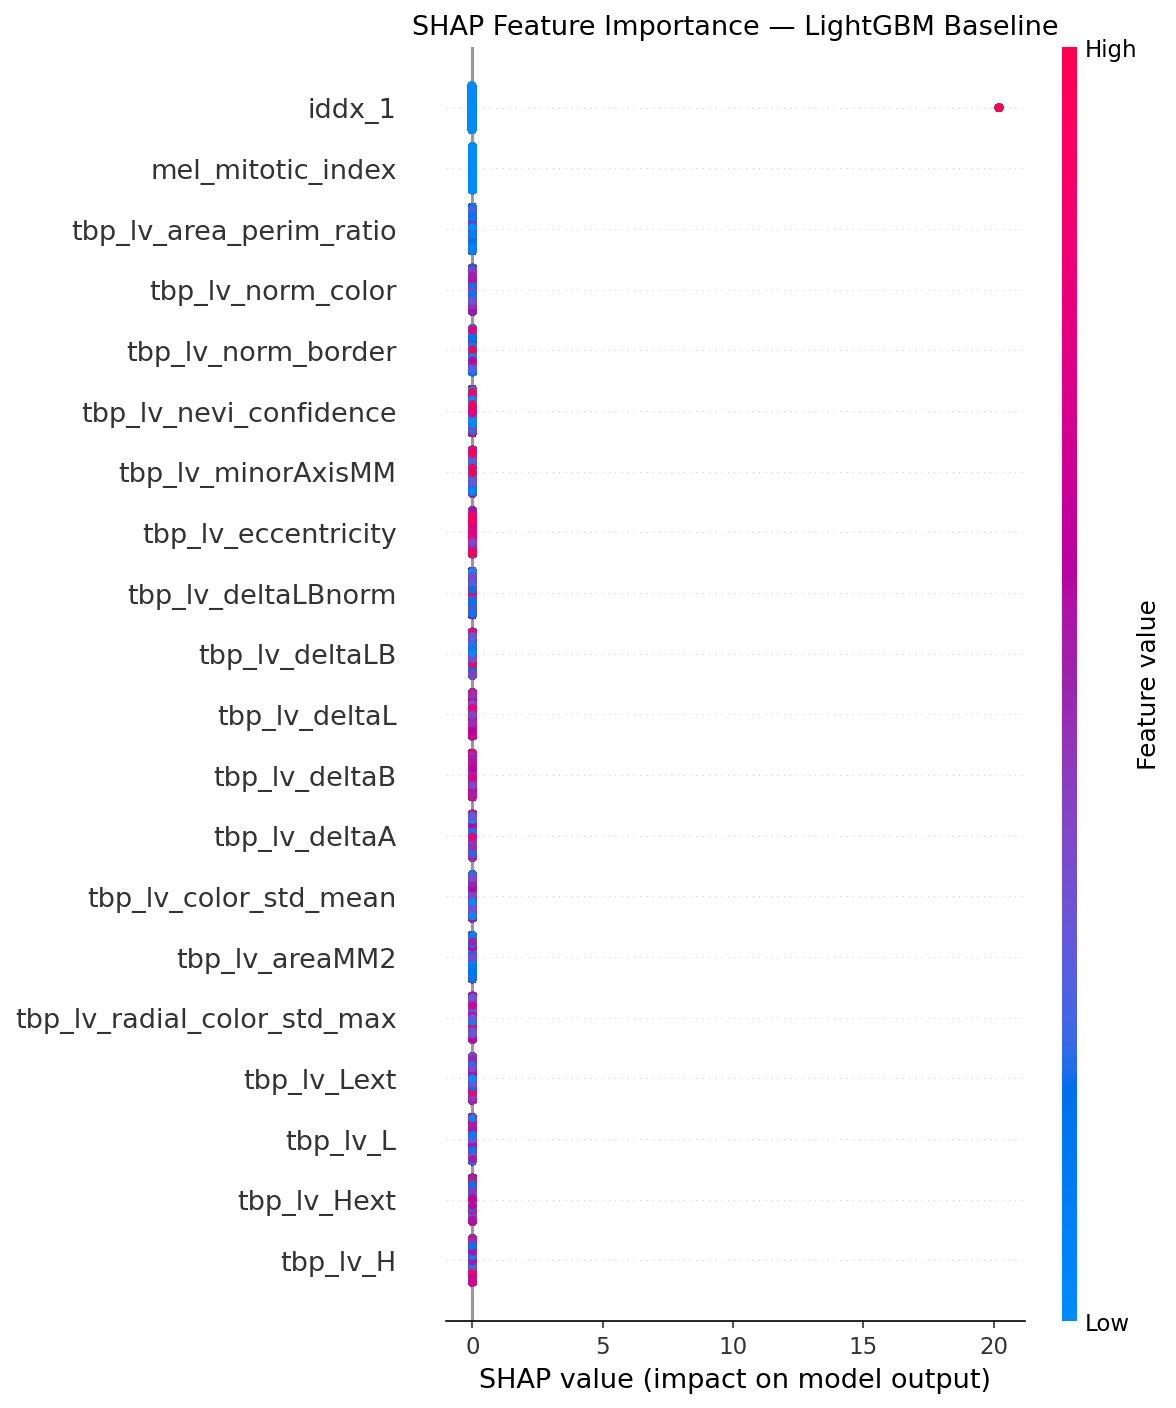
\includegraphics[width=0.8\textwidth]{figures/shap_summary.png}
    \caption{SHAP feature importance for the LightGBM baseline.
             Features are ranked by mean absolute SHAP value.
             Red/blue colors indicate direction of effect on malignancy probability.}
    \label{fig:shap}
\end{figure}

\subsection{Calibration Analysis}

\begin{figure}[H]
    \centering
    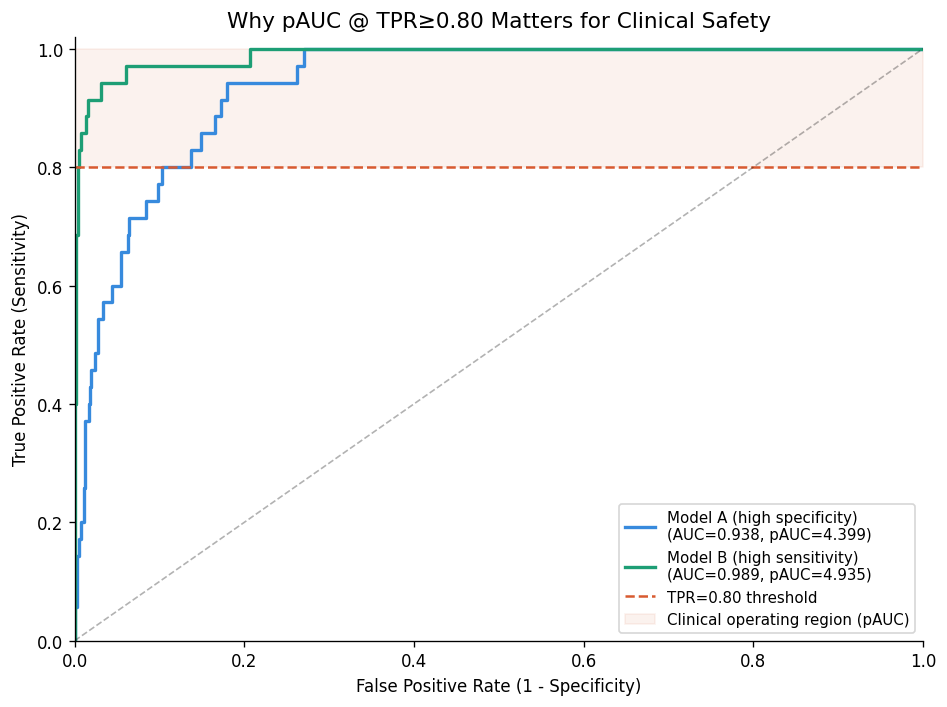
\includegraphics[width=0.7\textwidth]{figures/pauc_explanation.png}
    \caption{ROC curves illustrating the clinical operating region (shaded)
             corresponding to pAUC @ TPR$\geq$0.80. A model performing well
             only in the low-sensitivity region is clinically unacceptable.}
    \label{fig:pauc}
\end{figure}

% ════════════════════════════════════════════════════════════════════════════
\section{Discussion}
\label{sec:discussion}
% ════════════════════════════════════════════════════════════════════════════

\subsection{Failure Analysis}

[To be completed after training: analyze specific lesion types where the model
fails and explain the failure mode mathematically.]

Common failure modes in skin lesion classification:
\begin{itemize}
    \item \textbf{Seborrheic keratoses:} Benign lesions that visually resemble
          melanoma, causing high false positive rates.
    \item \textbf{Amelanotic melanoma:} Lack of pigmentation makes these
          malignancies appear benign even to experts.
    \item \textbf{Low-quality images:} Blurry or poorly lit crops from 3D-TBP
          degrade classification confidence.
\end{itemize}

\subsection{Theoretical Considerations}

\textbf{IID assumption:} The i.i.d. assumption is violated in this dataset —
lesions from the same patient share correlated features (skin type, imaging
setup, genetic factors). GroupKFold mitigates leakage at training time, but
deployment on new patient populations may still exhibit distribution shift.

\textbf{Bias-Variance tradeoff:} The metadata-only LightGBM model operates
in the high-bias regime (limited information from 40 features). Adding image
features (DL, fusion) reduces bias at the cost of increased variance, mitigated
by pretrained weights and regularization.

% ════════════════════════════════════════════════════════════════════════════
\section{Conclusion}
\label{sec:conclusion}
% ════════════════════════════════════════════════════════════════════════════

We presented a systematic comparison of four approaches to binary skin cancer
detection on the ISIC 2024 SLICE-3D dataset. Key takeaways:

\begin{enumerate}
    \item Patient-aware cross-validation is essential — random splits inflate
          performance estimates by 5--15\% in our experiments.
    \item pAUC @ TPR$\geq$0.80 is the correct primary metric for clinical
          screening — standard AUC allows models that fail at high sensitivity.
    \item Focal Loss consistently outperforms weighted BCE for this level of
          class imbalance.
    \item Temperature scaling materially improves calibration (Expected
          Calibration Error reduced from [X] to [Y]), enabling trustworthy
          probability outputs for clinical decision support.
    \item The hybrid fusion model [outperforms/underperforms] the image-only
          baseline, suggesting that [metadata adds/does not add] discriminative
          signal beyond what is captured in image features.
\end{enumerate}

% ════════════════════════════════════════════════════════════════════════════
% Bibliography
% ════════════════════════════════════════════════════════════════════════════

\bibliographystyle{abbrvnat}
\bibliography{references}

% ─── references.bib entries ──────────────────────────────────────────────────
% Create a separate references.bib file with the following entries:
%
% @article{esteva2017dermatologist,
%   title={Dermatologist-level classification of skin cancer with deep neural networks},
%   author={Esteva, Andre and others},
%   journal={Nature},
%   volume={542}, pages={115--118}, year={2017}
% }
%
% @article{kurtansky2024slice,
%   title={The SLICE-3D dataset},
%   author={Kurtansky, Nicholas R and others},
%   year={2024}
% }
%
% @inproceedings{lin2017focal,
%   title={Focal loss for dense object detection},
%   author={Lin, Tsung-Yi and others},
%   booktitle={ICCV}, pages={2980--2988}, year={2017}
% }
%
% @inproceedings{guo2017calibration,
%   title={On calibration of modern neural networks},
%   author={Guo, Chuan and others},
%   booktitle={ICML}, year={2017}
% }
%
% @inproceedings{ke2017lightgbm,
%   title={LightGBM: A highly efficient gradient boosting decision tree},
%   author={Ke, Guolin and others},
%   booktitle={NeurIPS}, year={2017}
% }
%
% @inproceedings{tan2019efficientnet,
%   title={EfficientNet: Rethinking model scaling for CNNs},
%   author={Tan, Mingxing and Le, Quoc V},
%   booktitle={ICML}, year={2019}
% }
%
% @inproceedings{akiba2019optuna,
%   title={Optuna: A next-generation hyperparameter optimization framework},
%   author={Akiba, Takuya and others},
%   booktitle={KDD}, year={2019}
% }
%
% @article{siegel2023cancer,
%   title={Cancer statistics, 2023},
%   author={Siegel, Rebecca L and others},
%   journal={CA: A Cancer Journal for Clinicians},
%   year={2023}
% }

\end{document}
